\subsection{Overlapping Subdomains}

\definition{Overlapping Subdomains} refer to the concept within Domain Decomposition Methods where the \textbf{computational domain is divided into smaller regions that share some common boundaries}. These shared boundaries are what make them \emph{overlapping}. This method is widely used to \textbf{enhance the convergence and accuracy of solving large-scale computational problems}, particularly partial differential equations (PDEs).

\highspace
\begin{flushleft}
    \textcolor{Green3}{\faIcon{tools} \textbf{Key Characteristics of Overlapping Subdomains}}
\end{flushleft}
\begin{enumerate}
    \item \textbf{Shared Boundaries}: The subdomains have regions where their boundaries overlap with adjacent subdomains. This overlapping region is critical for the exchange of information between subdomains.
    \item \textbf{Independent Solutions}: Each subdomain is solved independently, often in parallel, using updated boundary conditions from adjacent subdomains.
    \item \textbf{Iterative Process}: Solutions are updated iteratively by alternating between solving the subdomains and using the latest boundary conditions. This process continues until convergence is achieved.
\end{enumerate}

\begin{examplebox}
    Suppose we have a domain $\Omega$ that we want to solve a PDE on. We can divide $\Omega$ into two overlapping subdomains $\Omega_{1}$ and $\Omega_{2}$:
    \begin{itemize}
        \item Subdomain $\Omega_{1}$: Contains a portion of $\Omega$ and overlaps with $\Omega_{2}$ at the boundary.
        \item Subdomain $\Omega_{2}$: Contains another portion of $\Omega$ and overlaps with $\Omega_{1}$ at the boundary.
    \end{itemize}
\end{examplebox}

\highspace
\begin{flushleft}
    \textcolor{Green3}{\faIcon{check-circle} \textbf{Benefits of Overlapping Subdomains}}
\end{flushleft}
\begin{enumerate}
    \item \textbf{Improved Boundary Condition Handling}: The overlapping regions allow for better and more accurate boundary condition updates, leading to improved convergence rates.
    \item \textbf{Enhanced Convergence}: The iterative updates and information exchange in the overlapping regions help accelerate the convergence of the solution.
    \item \textbf{Parallel Processing}: Each subdomain can be solved independently, making it suitable for parallel computing, which significantly reduces computation time.
\end{enumerate}

\newpage

\subsubsection{Alternating Schwarz Method}

The \definition{Alternating Schwarz Method} is a classical \textbf{iterative technique} used in numerical linear algebra \textbf{to solve partial differential equations (PDEs)}. It is a type of domain decomposition method that divides the computational domain into overlapping subdomains.

\highspace
\begin{flushleft}
    \textcolor{Green3}{\faIcon{lightbulb} \textbf{Main idea}}
\end{flushleft}
\begin{itemize}
    \item \important{Domain Decomposition}: The main idea is to \textbf{break down a large problem into smaller, overlapping subproblems}. By solving these smaller problems iteratively, the overall solution can be efficiently approximated.
    \item \important{Overlap}: \textbf{Subdomains overlap at their boundaries}, allowing for more accurate boundary condition updates and improving the convergence rate of the method.
\end{itemize}

\highspace
\begin{flushleft}
    \textcolor{Green3}{\faIcon{tools} \textbf{Algorithm}}
\end{flushleft}
\begin{enumerate}
    \item \textbf{Initialization}: Start with an \emph{initial guess} for the solution over the entire domain.
    \item \textbf{Subdomain Solutions}: Alternately solve the PDE on each subdomain:
    \begin{itemize}
        \item On the first subdomain, using boundary conditions updated from the initial guess or the latest solution.
        \item On the second subdomain, using boundary conditions updated from the solution of the first subdomain.
    \end{itemize}
    \item \textbf{Iteration}: Continue alternating between subdomains, \textbf{updating the solution iteratively until convergence is achieved}.
\end{enumerate}

\highspace
\begin{examplebox}[: Elliptic Partial Differential Equation (PDE)]
    The problem involves solving an elliptic PDE of the form:
    \begin{equation*}
        Lu = f \hspace{1em} \text{in} \; \Omega = \Omega_{1} \cup \Omega_{2}
    \end{equation*}
    Where:
    \begin{itemize}
        \item $L$ is the \textbf{differential operator}.
        \item $u$ is the \textbf{unknown function we are solving for}.
        \item $f$ is a given function representing \textbf{the source term}.
        \item $\Omega$ is the \textbf{computational domain}, divided into two overlapping subdomains $\Omega_{1}$ and $\Omega_{2}$.
    \end{itemize}
    The boundary condition is:
    \begin{equation*}
        u = g \hspace{1em} \text{on} \; \partial \Omega
    \end{equation*}
    Here, $\partial \Omega$ represents the \textbf{boundary of the entire domain}.

    \highspace
    \textbf{Domain Decomposition}. The domain $\Omega$ is divided into two overlapping subdomains $\Omega_{1}$ and $\Omega_{2}$, each with its own boundary:
    \begin{itemize}
        \item $\Gamma_{1}$ is the boundary of $\Omega_{1}$.
        \item $\Gamma_{2}$ is the boundary of $\Omega_{2}$.
    \end{itemize}
    These subdomains overlap at certain regions, allowing for the exchange of boundary conditions and improving the overall convergence.
    \begin{center}
        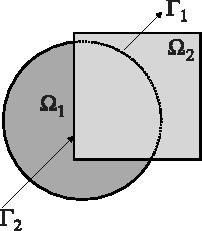
\includegraphics[width=.3\textwidth]{img/elliptic-pde-1.pdf}
    \end{center}

    \highspace
    \textbf{Iterative Solution Process}. The Alternating Schwarz Method iteratively solves the PDE on each subdomain while updating the boundary conditions based on the solutions from neighboring subdomains. The process involves the following steps:
    \begin{enumerate}
        \item \textbf{Initialization}. Start with an initial guess $ u^{(0)} $ for the solution.
        
        \item \textbf{Subdomain Solutions}:
        \begin{itemize}
            \item On $\Omega_{1}$:
            \begin{equation*}
                \begin{cases}
                    L u_{1}^{\left(k+\frac{1}{2}\right)} = f & \text{in} \; \Omega_{1} \vspace{.5em}\\
                    u_{1}^{\left(k+\frac{1}{2}\right)} = g & \text{on} \; \partial \Omega_{1} \setminus \Gamma_{1} \vspace{.5em}\\
                    u_{1}^{\left(k+\frac{1}{2}\right)} = u_{2}^{(k)} & \text{on} \; \Gamma_{1}
                \end{cases}
            \end{equation*}

            \item On $\Omega_{2}$:
            \begin{equation*}
                \begin{cases}
                    L u_{2}^{(k+1)} = f & \text{in} \; \Omega_{2} \vspace{.5em}\\
                    u_{2}^{(k+1)} = g & \text{on} \; \partial \Omega_{2} \setminus \Gamma_{2} \vspace{.5em}\\
                    u_{2}^{(k+1)} = u_{1}^{(k+\frac{1}{2})} & \text{on} \; \Gamma_{2}
                \end{cases}
            \end{equation*}
        \end{itemize}

        \item \textbf{Update}. Combine solutions to form the updated solution $u^{\left(k+1\right)}$:
        \begin{equation*}
            u^{(k+1)} =
            \begin{cases}
                u_{1}^{\left(k+\frac{1}{2}\right)} & \text{in} \; \Omega_{1} \setminus \Omega_{2} \vspace{.5em}\\
                u_{2}^{\left(k+1\right)} & \text{in} \; \Omega_{2}
            \end{cases}
        \end{equation*}
    \end{enumerate}

    \highspace
    \textbf{Convergence}. The iterative \textbf{process continues until the solutions on the overlapping subdomains converge to a stable solution for the entire domain} $\Omega$. The convergence rate is often enhanced due to the overlap and the iterative updating of boundary conditions.
\end{examplebox}